\documentclass[12pt, titlepage]{article}

\usepackage{fullpage}
\usepackage[round]{natbib}
\usepackage{multirow}
\usepackage{booktabs}
\usepackage{tabularx}
\usepackage{graphicx}
\usepackage{float}
\usepackage{hyperref}
\hypersetup{
    colorlinks,
    citecolor=blue,
    filecolor=black,
    linkcolor=red,
    urlcolor=blue
}

\usepackage{tikz}
\usetikzlibrary{arrows.meta,positioning}

\input{../../Comments}
%% Common Parts

\newcommand{\progname}{Software Engineering} % PUT YOUR PROGRAM NAME HERE
\newcommand{\authname}{Team 21, Visionaries
\\ Angela Zeng
\\ Ann Shi
\\ Ibrahim Sahi
\\ Manan Sharma
\\ Stanley Chen} % AUTHOR NAMES                  

\usepackage{hyperref}
    \hypersetup{colorlinks=true, linkcolor=blue, citecolor=blue, filecolor=blue,
                urlcolor=blue, unicode=false}
    \urlstyle{same}
                                


\newcounter{acnum}
\newcommand{\actheacnum}{AC\theacnum}
\newcommand{\acref}[1]{AC\ref{#1}}

\newcounter{ucnum}
\newcommand{\uctheucnum}{UC\theucnum}
\newcommand{\uref}[1]{UC\ref{#1}}

\newcounter{mnum}
\newcommand{\mthemnum}{M\themnum}
\newcommand{\mref}[1]{M\ref{#1}}

\begin{document}

\title{Module Guide for \progname{}} 
\author{\authname}
\date{\today}

\maketitle

\pagenumbering{roman}

\section{Revision History}

\begin{tabularx}{\textwidth}{p{3cm}p{2cm}X}
\toprule {\bf Date} & {\bf Version} & {\bf Notes}\\
\midrule
Nov. 13, 2025 & 1.0 & First revision of MG Document \\
Jan. 19, 2026 & 1.1 & Split privacy/infrastructure into single-secret modules; added uses DAG \\
\bottomrule
\end{tabularx}

\newpage

\section{Reference Material}

This section records information for easy reference.

\subsection{Abbreviations and Acronyms}

\renewcommand{\arraystretch}{1.2}
\begin{tabular}{l l} 
  \toprule		
  \textbf{symbol} & \textbf{description}\\
  \midrule 
  AC & Anticipated Change\\
  DAG & Directed Acyclic Graph \\
  M & Module \\
  MG & Module Guide \\
  OS & Operating System \\
  FR & Functional Requirement\\
  NFR & Non-Functional Requirement\\
  SC & Scientific Computing \\
  SRS & Software Requirements Specification\\
  \progname & Explanation of program name\\
  UC & Unlikely Change \\
  ET & Eye-tracking \\
  CI/CD & Continuous Integration / Continuous Delivery \\
  API & Application Programming Interface \\
  RBAC & Role-based Access Control \\
  POC & Proof-of-Concept \\
  \bottomrule
\end{tabular}\\

\newpage

\tableofcontents

\listoftables

\listoffigures

\newpage

\pagenumbering{arabic}

\section{Introduction}

Decomposing a system into modules is a commonly accepted approach to developing
software.  A module is a work assignment for a programmer or programming
team~\citep{ParnasEtAl1984}.  We advocate a decomposition
based on the principle of information hiding~\citep{Parnas1972a}.  This
principle supports design for change, because the ``secrets'' that each module
hides represent likely future changes.  Design for change is valuable in SC,
where modifications are frequent, especially during initial development as the
solution space is explored.  

Our design follows the rules layed out by \citet{ParnasEtAl1984}, as follows:
\begin{itemize}
\item System details that are likely to change independently should be the
  secrets of separate modules.
\item Each data structure is implemented in only one module.
\item Any other program that requires information stored in a module's data
  structures must obtain it by calling access programs belonging to that module.
\end{itemize}

After completing the first stage of the design, the Software Requirements
Specification (SRS), the Module Guide (MG) is developed~\citep{ParnasEtAl1984}. The MG
specifies the modular structure of the system and is intended to allow both
designers and maintainers to easily identify the parts of the software.  The
potential readers of this document are as follows:

\begin{itemize}
\item New project members: This document can be a guide for a new project member
  to easily understand the overall structure and quickly find the
  relevant modules they are searching for.
\item Maintainers: The hierarchical structure of the module guide improves the
  maintainers' understanding when they need to make changes to the system. It is
  important for a maintainer to update the relevant sections of the document
  after changes have been made.
\item Designers: Once the module guide has been written, it can be used to
  check for consistency, feasibility, and flexibility. Designers can verify the
  system in various ways, such as consistency among modules, feasibility of the
  decomposition, and flexibility of the design.
\end{itemize}

The rest of the document is organized as follows. Section
\ref{SecChange} lists the anticipated and unlikely changes of the software
requirements. Section \ref{SecMH} summarizes the module decomposition that
was constructed according to the likely changes. Section \ref{SecConnection}
specifies the connections between the software requirements and the
modules. Section \ref{SecMD} gives a detailed description of the
modules. Section \ref{SecTM} includes two traceability matrices. One checks
the completeness of the design against the requirements provided in the SRS. The
other shows the relation between anticipated changes and the modules. Section
\ref{SecUse} describes the use relation between modules.

\section{Anticipated and Unlikely Changes} \label{SecChange}

This section lists possible changes to the system. According to the likeliness
of the change, the possible changes are classified into two
categories. Anticipated changes are listed in Section \ref{SecAchange}, and
unlikely changes are listed in Section \ref{SecUchange}.

\subsection{Anticipated Changes} \label{SecAchange}

Anticipated changes are the source of the information that is to be hidden
inside the modules. Ideally, changing one of the anticipated changes will only
require changing the one module that hides the associated decision. The approach
adapted here is called design for
change.

\begin{description}
\item[\refstepcounter{acnum} \actheacnum \label{acDashboard}:] The design and presentation of output data may evolve as we introduce a dashboard for post-session and real-time analytics. Visualizations and their underlying implementations are expected to change based on usability feedback and new instructor needs.
\item[\refstepcounter{acnum} \actheacnum \label{acHomography}:] The current homography module is anticipated to be updated with lighter-weight or more efficient algorithms. These changes aim to improve alignment accuracy and reduce latency for real-time gaze projection.
\item[\refstepcounter{acnum} \actheacnum \label{acAnalytics}:] Additional analytics such as engagement metrics or anomaly detection may be added as part of the dashboard.
\item[\refstepcounter{acnum} \actheacnum \label{acPrivacy}:] Privacy, access-control, storage/retention, and monitoring policies may evolve (or be introduced) as we harden the system for classroom deployment and research compliance (e.g., redaction rules, RBAC roles, retention windows, audit logging).
\end{description}

\subsection{Unlikely Changes} \label{SecUchange}

The module design should be as general as possible. However, a general system is
more complex. Sometimes this complexity is not necessary. Fixing some design
decisions at the system architecture stage can simplify the software design. If
these decision should later need to be changed, then many parts of the design
will potentially need to be modified. Hence, it is not intended that these
decisions will be changed.

\begin{description}
\item[\refstepcounter{ucnum} \uctheucnum \label{ucHardware}:] The existing system relies on fixed hardware (Pupil Labs Neon Eye Tracking Glasses, Android smartphone, network webcam), and changing these devices would require extensive redesign. 
\item[\refstepcounter{ucnum} \uctheucnum \label{ucAPIs}:] The pipeline depends heavily on Pupil Labs’ APIs for data access and synchronization. Modifying or replacing these APIs would impact multiple system components, making such changes unlikely.
\item[\refstepcounter{ucnum} \uctheucnum \label{ucInput}:] The system assumes specific input data formats. Altering these formats would require large-scale changes to parsing and processing modules.
\item[\refstepcounter{ucnum} \uctheucnum \label{ucCLI}:] The existing CLI supports essential homography, visualization, and analysis functions. Its role in offline processing makes major changes unlikely.
\item[\refstepcounter{ucnum} \uctheucnum \label{ucGlassesRecordModule}:] The existing GlassesRecord module handles multi-glasses recording and synchronization through a custom terminal interface will most likely not be changed. 
\end{description}

\section{Module Hierarchy} \label{SecMH}

This section provides an overview of the module design. Modules are summarized
in a hierarchy decomposed by secrets in Table \ref{TblMH}. The modules listed
below, which are leaves in the hierarchy tree, are the modules that will
actually be implemented.

\begin{description}
  \item[\refstepcounter{mnum} \mthemnum \label{mHH}:] Hardware-Hiding Module
  \item[\refstepcounter{mnum} \mthemnum \label{mDIM}:] Data Ingestion Module
  \item[\refstepcounter{mnum} \mthemnum \label{mRTS}:] Real-Time Streaming Module
  \item[\refstepcounter{mnum} \mthemnum \label{mDVM}:] Dashboard Visualization Module
  \item[\refstepcounter{mnum} \mthemnum \label{mRM}:] Reporting Module
  \item[\refstepcounter{mnum} \mthemnum \label{mDPM}:] Data Preprocessing Module

  \item[\refstepcounter{mnum} \mthemnum \label{mPFM}:] Privacy Filtering Module
  \item[\refstepcounter{mnum} \mthemnum \label{mACM}:] Access Control Module
  \item[\refstepcounter{mnum} \mthemnum \label{mSRM}:] Secure Storage \& Retention Module
  \item[\refstepcounter{mnum} \mthemnum \label{mOM}:] Observability Module

  \item[\refstepcounter{mnum} \mthemnum \label{mEAM}:] Engagement Analytics Module
  \item[\refstepcounter{mnum} \mthemnum \label{mCVAM}:] Correlation \& Visual Analysis Module
\end{description}

\begin{table}[h!]
\centering
\begin{tabular}{p{0.3\textwidth} p{0.6\textwidth}}
\toprule
\textbf{Level 1} & \textbf{Level 2}\\
\midrule

Hardware-Hiding Module & Hardware-Hiding Module (\mref{mHH}) \\
\midrule

\multirow{4}{0.3\textwidth}{Behaviour-Hiding Module} 
  & Data Ingestion Module (\mref{mDIM})\\
  & Real-Time Streaming Module (\mref{mRTS})\\
  & Dashboard Visualization Module (\mref{mDVM})\\
  & Reporting Module (\mref{mRM})\\
\midrule

\multirow{7}{0.3\textwidth}{Software Decision Module} 
  & Data Preprocessing Module (\mref{mDPM})\\
  & Privacy Filtering Module (\mref{mPFM})\\
  & Access Control Module (\mref{mACM})\\
  & Secure Storage \& Retention Module (\mref{mSRM})\\
  & Observability Module (\mref{mOM})\\
  & Engagement Analytics Module (\mref{mEAM})\\
  & Correlation \& Visual Analysis Module (\mref{mCVAM})\\
\bottomrule

\end{tabular}
\caption{Module Hierarchy}
\label{TblMH}
\end{table}

\section{Connection Between Requirements and Design} \label{SecConnection}

The design of the system is intended to satisfy the requirements developed in
the SRS. In this stage, the system is decomposed into modules. The connection
between requirements and modules is listed in Table~\ref{TblRT}.

\begin{itemize}

  \item \textbf{Separation of data ingestion from preprocessing:}
  Requirements relating to multi-device input, raw data capture, timing
  synchronization, and recovery from connection loss motivated the creation of a
  dedicated \emph{Data Ingestion Module}. Requirements concerning noise
  reduction, calibration correction, homography projection, and coordinate
  normalization are distinct and subject to change independently, motivating the
  \emph{Data Preprocessing Module}. This reflects the SRS separation between raw
  data capture and analytic data preparation.

  \item \textbf{Explicit handling of real-time constraints:}
  The need for live metrics, dashboard updating, latency guarantees, and
  real-time streaming (as described in the SRS operational modes) led to the
  creation of a separate \emph{Real-Time Streaming Module}. This encapsulates
  decisions about streaming frameworks, buffering policy, and delivery latency,
  which are likely to evolve as performance constraints change.

  \item \textbf{Distinguishing analytics computation from visualization:}
  Engagement metrics, instructor–student gaze alignment, heatmap generation,
  and correlation analyses are internal computations not directly described to
  the end user. These behaviours motivated two separate software-decision
  modules: the \emph{Engagement Analytics Module} and the \emph{Correlation \&
  Visual Analysis Module}. Meanwhile, all visible UI behaviours—including
  real-time views, playback, filtering, and seat-map interactions—are grouped in
  the \emph{Dashboard Visualization Module}. This follows the SRS distinction
  between analytic computation and user-facing presentation.

  \item \textbf{Privacy as a first-class design concern (split into independent secrets):}
  The SRS includes privacy/anonymization, RBAC access control, secure storage/retention,
  and logging/monitoring requirements. These concerns change independently and
  should not be embedded inside ingestion, analytics, or dashboard logic without
  creating strong coupling. Therefore, the former monolithic ``Privacy \& Infrastructure''
  responsibility is decomposed into:
  \begin{itemize}
    \item \emph{Privacy Filtering Module} for redaction/anonymization rules,
    \item \emph{Access Control Module} for RBAC/authz policy,
    \item \emph{Secure Storage \& Retention Module} for storage schema/retention strategy,
    \item \emph{Observability Module} for audit logging/monitoring configuration.
  \end{itemize}

  \item \textbf{Support for offline summaries and instructor reporting:}
  Requirements calling for post-session summaries, exportable metrics, and
  instructor-friendly performance reports lead to the \emph{Reporting Module}.
  This module encapsulates decisions about report structure, export format, and
  summarization logic—decisions that are likely to change independently of both
  preprocessing and dashboard design.

  \item \textbf{Abstraction of physical devices and OS services:}
  The SRS assumes multiple hardware sources (eye-tracking glasses, central
  camera, audio, file storage, and network interfaces). To prevent downstream
  modules from depending on specific device drivers or OS-level behaviour, a
  general \emph{Hardware-Hiding Module} is included.

  \item \textbf{Backend service and session-lifecycle requirements:}
  The SRS specifies requirements for creating, managing, and retrieving recorded
  sessions, as well as backend API access for live or historical data. These behaviours
  are encapsulated in the \emph{Real-Time Streaming Module}, which provides client
  subscription and session-control interfaces.

\end{itemize}

Overall, the module structure shows the boundaries between behaviours visible
to the user, performance-driven internal computations, privacy-critical
infrastructure, and hardware-specific interactions. This makes sure that changes in
requirements - such as improved analytics, new privacy constraints, or new
hardware - affect only the module that hides the corresponding decision.

\section{Module Decomposition} \label{SecMD}

Modules are decomposed according to the principle of ``information hiding''
proposed by \citet{ParnasEtAl1984}. The \emph{Secrets} field in a module
decomposition is a brief statement of the design decision hidden by the
module. The \emph{Services} field specifies \emph{what} the module will do
without documenting \emph{how} to do it. For each module, a suggestion for the
implementing software is given under the \emph{Implemented By} title. If the
entry is \emph{OS}, this means that the module is provided by the operating
system or by standard programming language libraries.  \emph{\progname{}} means the
module will be implemented by the \progname{} software.

Only the leaf modules in the hierarchy have to be implemented. If a dash
(\emph{--}) is shown, this means that the module is not a leaf and will not have
to be implemented.

\subsection{Hardware Hiding Module (\mref{mHH})}

\begin{description}
\item[Secrets:] The device-specific interfaces, drivers, and low-level OS
mechanisms used to access eye-tracking glasses (Neon), world camera
input, microphones, GPU acceleration, file system APIs, local and cloud
storage backends, network sockets, and system time synchronization (e.g.,
NTP services).
\item[Services:] Provides a virtualized hardware interface for capturing gaze
streams, world camera frames, audio signals, timestamps, and device metadata,
and for reading/writing data to persistent storage. Exposes uniform APIs so
downstream modules do not depend on specific device models, storage engines,
or operating systems.
\item[Implemented By:] OS, vendor SDKs, device drivers
\item[Type of Module:] Library
\end{description}

\subsection{Behaviour-Hiding Modules}

\begin{description}
\item[Secrets:] The externally visible behaviours of the system, including
session playback, dashboard display logic, ingestion behaviour, and reporting
rules as defined in the SRS.
\item[Services:] Provides all user-facing behaviours, connecting virtualized
hardware to internal algorithms. These modules must change if the SRS behaviour
changes.
\item[Implemented By:] --
\end{description}

\subsubsection{Data Ingestion Module (\mref{mDIM})}

\begin{description}
\item[Secrets:] The method of connecting to and receiving data from multiple
hardware sources (glasses, cameras, microphones), including device protocols,
buffering policy, timestamp alignment strategy (including use of system/NTP
time), and fault-recovery behaviour for dropped connections or device failures.
\item[Services:]
\begin{itemize}
  \item Accepts raw gaze, video, audio, and metadata streams from all devices.
  \item Performs initial timestamping and session indexing using a common time
        base.
  \item Manages session start/stop hooks that allow backend services to create
        sessions, register participants, and mark completed recordings.
  \item Outputs unified raw data packets for preprocessing and optional storage.
\end{itemize}
\item[Implemented By:] \progname{}
\item[Type of Module:] Abstract Object
\end{description}

\subsubsection{Real-Time Streaming Module (\mref{mRTS})}

\begin{description}
\item[Secrets:] The design decisions for real-time transport, encrypted communication,
latency buffering, session lifecycle APIs, and authenticated endpoint access.
\item[Services:]
\begin{itemize}
  \item Exposes programmatic APIs for session creation, control, and analytics retrieval.
  \item Streams live and replay data using encrypted protocols.
  \item Enforces RBAC-protected access to all streaming and analytics endpoints.
  \item Maintains session state and reports health metrics to observability infrastructure.
\end{itemize}
\item[Implemented By:] \progname{}
\item[Type of Module:] Abstract Object
\end{description}

\subsubsection{Dashboard Visualization Module (\mref{mDVM})}

\begin{description}
\item[Secrets:] The visualization grammar, UI layout, interaction rules,
role-based presentation logic, and display of system status indicators.
\item[Services:]
\begin{itemize}
  \item Presents real-time and historical analytics.
  \item Renders heatmaps, fixation charts, engagement timelines, and gaze-alignment plots.
  \item Displays system status indicators (latency, stream health, sync drift).
  \item Supports role-based views (e.g., instructor vs.\ researcher).
  \item Provides playback and filtering over recorded sessions.
\end{itemize}
\item[Implemented By:] \progname{}
\item[Type of Module:] Abstract Object
\end{description}

\subsubsection{Reporting Module (\mref{mRM})}

\begin{description}
\item[Secrets:] The structure and formatting of summaries, metrics, annotations,
and export formats (CSV, JSON, PNG) and the rules for instructor reflection and research reporting.
\item[Services:]
\begin{itemize}
  \item Generates post-session summaries and aggregated attention metrics.
  \item Exports analytics and visualizations in CSV, JSON, and PNG formats.
  \item Supports annotation, note-taking, and timeline cropping for instructional review.
\end{itemize}
\item[Implemented By:] \progname{}
\item[Type of Module:] Library
\end{description}

\subsection{Software Decision Modules}

\begin{description}
\item[Secrets:] Internal algorithms, mathematical models, data structures, and
analytic methods that are not externally visible. These change primarily due to
performance or research-driven improvements, not due to changes in behaviour.
\item[Services:] Provides internal data processing, analytics, correlations, and
privacy enforcement services for behaviour-hiding modules.
\item[Implemented By:] --
\end{description}

\subsubsection{Data Preprocessing Module (\mref{mDPM})}

\begin{description}
\item[Secrets:] Filtering algorithms (smoothing, denoising), calibration
transformations, gaze-to-screen homography methods, fixation detection rules,
and temporal alignment techniques.
\item[Services:]
\begin{itemize}
  \item Converts raw gaze vectors into screen/world-space coordinates.
  \item Denoises and filters gaze data.
  \item Identifies fixations, saccades, attention windows.
  \item Standardizes multimodal streams for analytics.
\end{itemize}
\item[Implemented By:] \progname{}
\item[Type of Module:] Abstract Data Type
\end{description}

\subsubsection{Privacy Filtering Module (\mref{mPFM})}

\begin{description}
\item[Secrets:] The anonymization and redaction policy applied to video, gaze data,
stored artifacts, and exported outputs.
\item[Services:]
\begin{itemize}
  \item Applies redaction and masking rules to raw and derived data.
  \item Ensures masked regions are excluded prior to storage and export.
  \item Removes or obfuscates identifiers from analytics and reports.
\end{itemize}
\item[Implemented By:] \progname{}
\item[Type of Module:] Library
\end{description}


\subsubsection{Access Control Module (\mref{mACM})}

\begin{description}
\item[Secrets:] Authentication strategy and RBAC policy for dashboards, analytics,
streaming APIs, and data exports.
\item[Services:]
\begin{itemize}
  \item Authenticates users and services.
  \item Authorizes access to dashboards, analytics APIs, and exports based on role.
\end{itemize}
\item[Implemented By:] \progname{}
\item[Type of Module:] Library
\end{description}

\subsubsection{Secure Storage \& Retention Module (\mref{mSRM})}

\begin{description}
\item[Secrets:] Storage backend selection, encryption-at-rest strategy,
session metadata schema, retention windows, and traceability linkage rules.
\item[Services:]
\begin{itemize}
  \item Stores raw, anonymized, and processed session artifacts.
  \item Stores session metadata (session ID, timestamps, participant mappings).
  \item Maintains traceability links between raw data, analytics, and reports.
  \item Enforces retention and deletion policies.
\end{itemize}
\item[Implemented By:] \progname{}
\item[Type of Module:] Abstract Data Type
\end{description}

\subsubsection{Observability Module (\mref{mOM})}

\begin{description}
\item[Secrets:] Audit logging policy and performance metric definitions.
\item[Services:]
\begin{itemize}
  \item Records audit logs for access and export actions.
  \item Collects runtime metrics (latency, dropped frames, sync drift).
  \item Exposes metrics used by dashboard status indicators.
\end{itemize}
\item[Implemented By:] \progname{}
\item[Type of Module:] Library
\end{description}

\subsubsection{Engagement Analytics Module (\mref{mEAM})}

\begin{description}
\item[Secrets:] The mathematical models used to compute engagement metrics,
moving averages, attention peaks/troughs, activity-phase detection, and time-on-task calculations.
\item[Services:]
\begin{itemize}
  \item Computes engagement over time for individuals and aggregates.
  \item Detects disengagement periods and high-attention intervals.
  \item Classifies lecture activities (discussion, slides, group work).
  \item Generates metrics for reporting and dashboard visualization.
\end{itemize}
\item[Implemented By:] \progname{}
\item[Type of Module:] Abstract Data Type
\end{description}

\subsubsection{Correlation \& Visual Analysis Module (\mref{mCVAM})}

\begin{description}
\item[Secrets:] The gaze-correlation model, instructor–student alignment formulas,
visual material detection (text block, image region), and methods for transforming
heatmaps into interpretable coordinate-space analytics.
\item[Services:]
\begin{itemize}
  \item Computes correlations between instructor gaze and class gaze.
  \item Maps class attention onto slide regions or world-camera space.
  \item Identifies which visual elements students focus on, and how this changes over time.
  \item Supports seat-map and spatial-zone based metrics and filters.
\end{itemize}
\item[Implemented By:] \progname{}
\item[Type of Module:] Abstract Data Type
\end{description}

\section{Traceability Matrix} \label{SecTM}

This section shows two traceability matrices: between the modules and the
requirements and between the modules and the anticipated changes.

\begin{table}[H]
\centering
\begin{tabular}{p{0.2\textwidth} p{0.6\textwidth}}
\toprule
\textbf{Req.} & \textbf{Modules}\\
\midrule
FR-10 & \mref{mEAM}, \mref{mCVAM}, \mref{mRM}, \mref{mDVM} \\
FR-11 & \mref{mSRM} \\
FR-12 & \mref{mDIM}, \mref{mSRM} \\
FR-13 & \mref{mRTS}, \mref{mACM} \\
FR-14 & \mref{mACM} \\
FR-17 & \mref{mDVM}, \mref{mACM} \\
FR-18 & \mref{mOM} \\
FR-21 & \mref{mPFM}, \mref{mRTS}, \mref{mSRM} \\
FR-22 & \mref{mSRM}, \mref{mRM} \\
FR-26 & \mref{mDVM}, \mref{mOM}, \mref{mRTS} \\
FR-27 & \mref{mPFM}, \mref{mSRM}, \mref{mRM} \\
NFR-9 & \mref{mRTS}, \mref{mSRM} \\
NFR-10 & \mref{mACM}, \mref{mRTS}, \mref{mDVM} \\
NFR-11 & \mref{mPFM}, \mref{mSRM} \\
\bottomrule
\end{tabular}
\caption{Trace Between Requirements and Modules}
\label{TblRT}
\end{table}

\begin{table}[H]
\centering
\begin{tabular}{p{0.2\textwidth} p{0.6\textwidth}}
\toprule
\textbf{AC} & \textbf{Modules}\\
\midrule
\acref{acDashboard} & \mref{mDVM}, \mref{mRM}, \mref{mDPM}, \mref{mEAM}, \mref{mCVAM} \\
\acref{acHomography} & \mref{mRTS}, \mref{mDPM} \\
\acref{acAnalytics} & \mref{mEAM}, \mref{mCVAM}, \mref{mDVM}, \mref{mRM} \\
\acref{acPrivacy} & \mref{mPFM}, \mref{mACM}, \mref{mSRM}, \mref{mOM} \\
\bottomrule
\end{tabular}
\caption{Trace Between Anticipated Changes and Modules}
\label{TblACT}
\end{table}

\section{Use Hierarchy Between Modules} \label{SecUse}

In this section, the uses hierarchy between modules is
provided. \citet{Parnas1978} said of two programs A and B that A {\em uses} B if
correct execution of B may be necessary for A to complete the task described in
its specification. That is, A {\em uses} B if there exist situations in which
the correct functioning of A depends upon the availability of a correct
implementation of B. Figure \ref{FigUH} summarizes the use relation between the
modules as a directed acyclic graph (DAG). The edge list below is a readable
restatement of the same relations.

At a high level, the use hierarchy for \progname{} is organized into layers:

\begin{itemize}
  \item \textbf{Level 0 – Hardware layer}: 
  Hardware-Hiding Module (\mref{mHH}) encapsulates device/OS access. No other module is used by \mref{mHH}.

  \item \textbf{Level 1 – Data acquisition}: 
  Data Ingestion Module (\mref{mDIM}) uses \mref{mHH} to collect raw gaze and video streams.

  \item \textbf{Level 2 – Preparation}: 
  Data Preprocessing Module (\mref{mDPM}) uses \mref{mDIM} to filter, normalize, and structure captured data.

  \item \textbf{Level 2 – Cross-cutting governance}: 
  Privacy Filtering (\mref{mPFM}) uses \mref{mDIM} and \mref{mDPM} to enforce redaction rules.
  Access Control (\mref{mACM}) provides authorization checks to protect API and session actions.
  Secure Storage \& Retention (\mref{mSRM}) uses \mref{mDIM}, \mref{mDPM}, and \mref{mPFM} to store and retrieve privacy-compliant artifacts and enforce retention policies.
  Observability (\mref{mOM}) collects logs and runtime metrics from other modules.

  \item \textbf{Level 3 – Analytics and streaming}: 
  Real-Time Streaming (\mref{mRTS}) uses \mref{mDIM}, \mref{mDPM}, and governance modules to serve compliant streams.
  Engagement Analytics (\mref{mEAM}) uses \mref{mDPM}.
  Correlation \& Visual Analysis (\mref{mCVAM}) uses \mref{mDPM} and \mref{mEAM}.

  \item \textbf{Level 4 – User-facing visualization}: 
  Dashboard Visualization (\mref{mDVM}) uses \mref{mRTS}, \mref{mEAM}, \mref{mCVAM}, \mref{mACM}, and \mref{mOM}.

  \item \textbf{Level 5 – Reporting and exports}: 
  Reporting (\mref{mRM}) uses \mref{mDVM}, \mref{mEAM}, \mref{mCVAM}, \mref{mSRM}, and \mref{mACM}.
\end{itemize}

\begin{figure}[H]
\centering
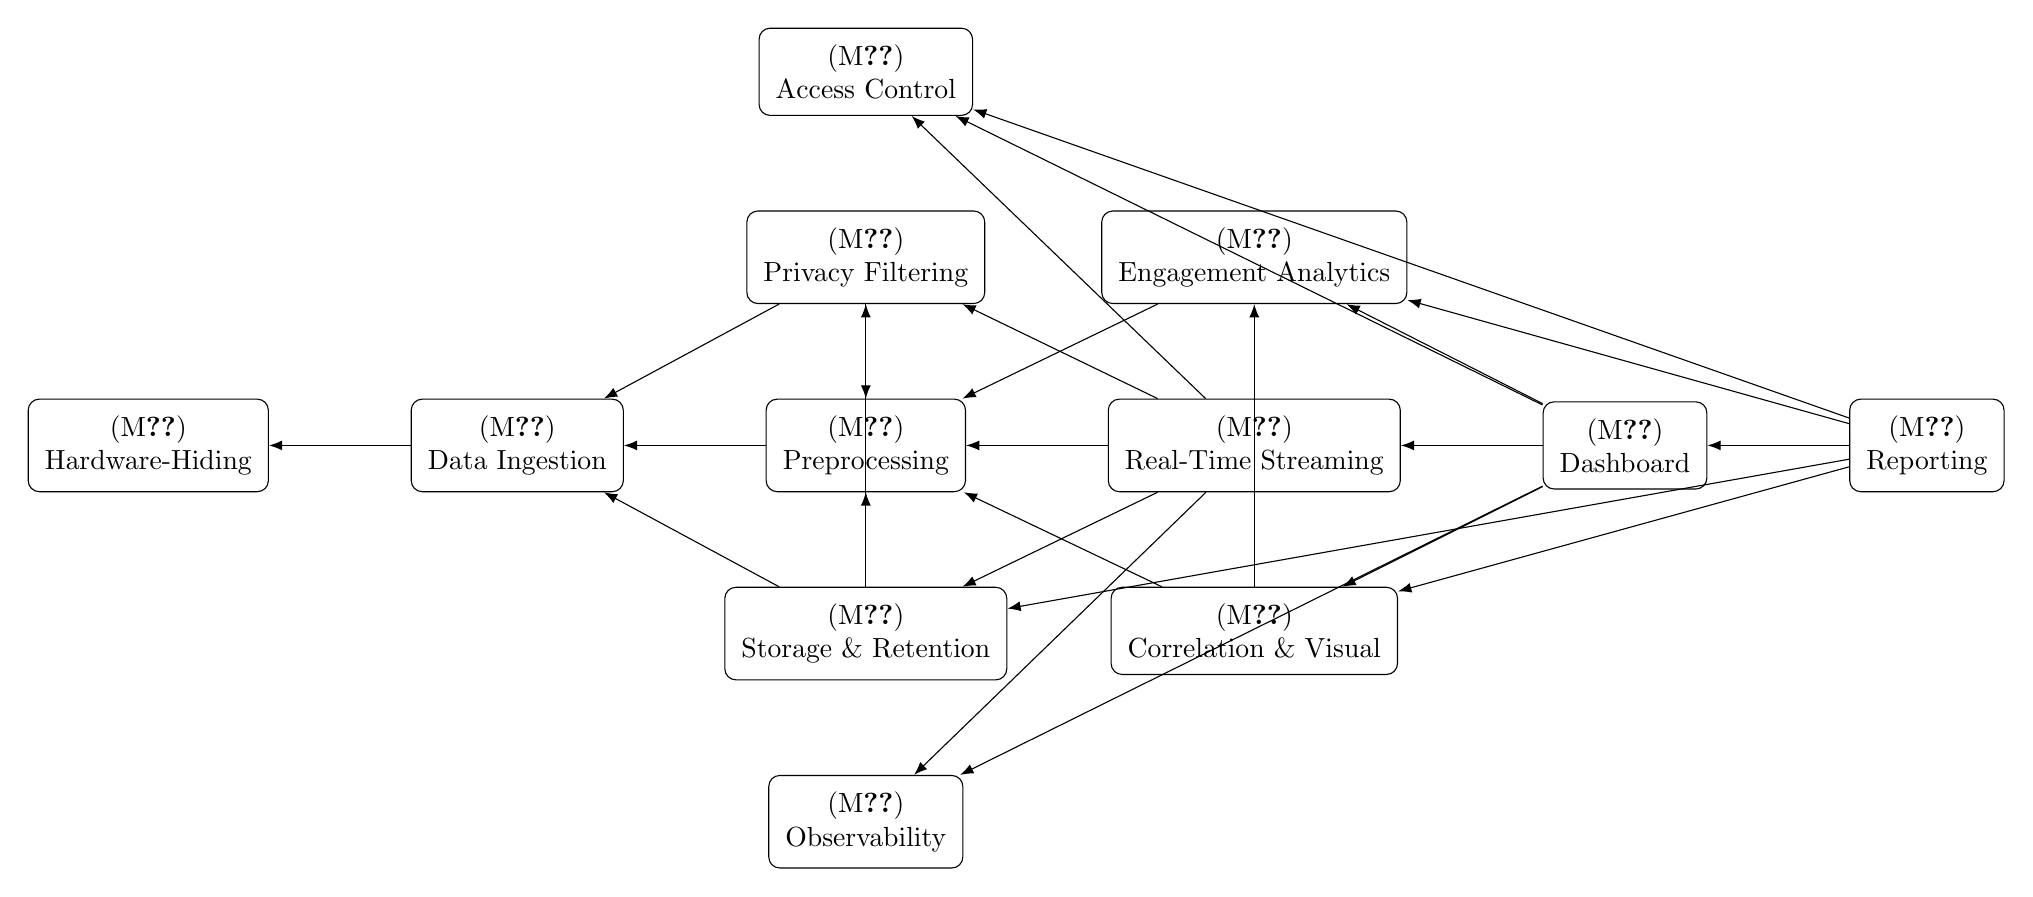
\begin{tikzpicture}[
  node distance=1.2cm and 1.8cm,
  box/.style={draw, rounded corners, align=center, inner sep=6pt},
  arrow/.style={-Latex}
]
\node[box] (m1) {(\mref{mHH})\\Hardware-Hiding};
\node[box, right=of m1] (m2) {(\mref{mDIM})\\Data Ingestion};
\node[box, right=of m2] (m6) {(\mref{mDPM})\\Preprocessing};

\node[box, above=of m6] (m7a) {(\mref{mPFM})\\Privacy Filtering};
\node[box, above=of m7a] (m7b) {(\mref{mACM})\\Access Control};
\node[box, below=of m6] (m7c) {(\mref{mSRM})\\Storage \& Retention};
\node[box, below=of m7c] (m7d) {(\mref{mOM})\\Observability};

\node[box, right=of m6] (m3) {(\mref{mRTS})\\Real-Time Streaming};
\node[box, above=of m3] (m8) {(\mref{mEAM})\\Engagement Analytics};
\node[box, below=of m3] (m9) {(\mref{mCVAM})\\Correlation \& Visual};

\node[box, right=of m3] (m4) {(\mref{mDVM})\\Dashboard};
\node[box, right=of m4] (m5) {(\mref{mRM})\\Reporting};

\draw[arrow] (m2) -- (m1);
\draw[arrow] (m6) -- (m2);

\draw[arrow] (m7a) -- (m6);
\draw[arrow] (m7c) -- (m6);

\draw[arrow] (m3) -- (m6);
\draw[arrow] (m3) -- (m7a);
\draw[arrow] (m3) -- (m7b);
\draw[arrow] (m3) -- (m7c);
\draw[arrow] (m3) -- (m7d);

\draw[arrow] (m8) -- (m6);
\draw[arrow] (m9) -- (m6);
\draw[arrow] (m9) -- (m8);

\draw[arrow] (m4) -- (m3);
\draw[arrow] (m4) -- (m8);
\draw[arrow] (m4) -- (m9);
\draw[arrow] (m4) -- (m7b);

\draw[arrow] (m5) -- (m4);
\draw[arrow] (m5) -- (m8);
\draw[arrow] (m5) -- (m9);
\draw[arrow] (m5) -- (m7c);
\draw[arrow] (m5) -- (m7b);
\draw[arrow] (m7a) -- (m2);
\draw[arrow] (m7c) -- (m2);
\draw[arrow] (m4) -- (m7d);
\draw[arrow] (m7c) -- (m7a);
\end{tikzpicture}
\caption{Use hierarchy among modules (DAG)}
\label{FigUH}
\end{figure}

The main uses relations can be summarized as:

\begin{itemize}
  \item \mref{mDIM} uses \mref{mHH}.
  \item \mref{mDPM} uses \mref{mDIM}.
  \item \mref{mPFM} uses \mref{mDIM} and \mref{mDPM}.
  \item \mref{mSRM} uses \mref{mDIM}, \mref{mDPM}, and \mref{mPFM}.
  \item \mref{mRTS} uses \mref{mDIM}, \mref{mDPM}, \mref{mPFM}, \mref{mACM}, \mref{mSRM}, and \mref{mOM}.
  \item \mref{mEAM} uses \mref{mDPM}.
  \item \mref{mCVAM} uses \mref{mDPM} and \mref{mEAM}.
  \item \mref{mDVM} uses \mref{mRTS}, \mref{mACM}, \mref{mOM}, \mref{mEAM}, and \mref{mCVAM}.
  \item \mref{mRM} uses \mref{mDVM}, \mref{mACM}, \mref{mSRM}, \mref{mEAM}, and \mref{mCVAM}.
\end{itemize}

\section{User Interfaces}

This section provides conceptual sketches of the primary user interface screens
for \progname{}. These sketches represent the core interactions and visual layout
of the system. They are intended to illustrate how instructors will navigate
through the platform, monitor real-time classroom attention, and review analytics
after each session. The sketches are early design mockups and may evolve as the
implementation progresses.

\subsection{10.1 Student Overview}

\begin{figure}[H]
\centering
\includegraphics[width=0.55\textwidth]{figure/Student_Overview.png}
\caption{Student Overview Screen}
\label{fig:student-overview}
\end{figure}

This screen serves as the entry point to the platform. Instructors can begin a
new live session or review summaries of previously recorded sessions.

\subsection{10.2 Live Classroom Dashboard}

\begin{figure}[H]
\centering
\includegraphics[width=0.55\textwidth]{figure/Live-Classroom-Dashboard.png}
\caption{Live Classroom Dashboard}
\label{fig:live-dashboard}
\end{figure}

During an active session, instructors are presented with a real-time dashboard.
It displays the recording state, a live camera feed from the capture device, and
a heatmap preview showing the current distribution of gaze activity.

\subsection{10.3 Student Attention Panel}

\begin{figure}[H]
\centering
\includegraphics[width=0.55\textwidth]{figure/Student_Attention_Panel.png}
\caption{Student Attention Panel}
\label{fig:student-attention-panel}
\end{figure}

This panel provides a real-time overview of individual student attention levels.
Each student is listed with a visual bar indicator, allowing the instructor to
quickly identify who is highly engaged, who is disengaged, and how attention
varies across learners.

\subsection{10.4 Selected Student Detail View}

\begin{figure}[H]
\centering
\includegraphics[width=0.55\textwidth]{figure/Selected_Student.png}
\caption{Selected Student Detail View}
\label{fig:selected-student}
\end{figure}

When a specific student is selected, the instructor is shown a detailed breakdown
of that student’s gaze distribution across key classroom regions (e.g., board,
instructor, walls). A small trend graph summarizes how their engagement changes
over time.

\subsection{10.5 Region-of-Interest Analytics}

\begin{figure}[H]
\centering
\includegraphics[width=0.55\textwidth]{figure/Region_of_Interest_Analytics.png}
\caption{Region-of-Interest (ROI) Analytics}
\label{fig:roi-analytics}
\end{figure}

This screen provides a post-session analytical view of where attention was
distributed in the classroom. Percentages for each region-of-interest are listed,
and an accompanying graph displays temporal patterns. Instructors may also toggle
visual elements such as scanpaths.

\subsection{10.6 Session Summary}

\begin{figure}[H]
\centering
\includegraphics[width=0.55\textwidth]{figure/Session_Summary.png}
\caption{Session Summary Screen}
\label{fig:session-summary}
\end{figure}

After a session ends, the summary view presents key metrics, including duration,
overall engagement, and the periods of highest attention. Instructors may export
a report for documentation or further analysis.

\subsection{10.7 Settings \& Calibration}

\begin{figure}[H]
\centering
\includegraphics[width=0.55\textwidth]{figure/Settings_Calibration.png}
\caption{Settings and Calibration Screen}
\label{fig:settings-calibration}
\end{figure}

The settings screen allows instructors to calibrate their eye-tracking device,
check battery level, test the camera feed, and adjust privacy or data storage
preferences. This screen ensures that sessions begin with reliable and
well-initialized hardware.

\section{Design of Communication Protocols}

This section describes the communication protocols used within \progname{}. 
Communication occurs between the client-facing dashboard, the real-time 
streaming backend, the analytics components, and the system’s secure storage 
infrastructure. All communication follows a modular service-based pattern 
where each module exposes a set of services that may be invoked by higher-level 
modules as shown in the uses hierarchy.

\subsection{11.1 Overall Architecture}

System communication is organized around three main channels:

\begin{itemize}
  \item \textbf{Real-Time Data Delivery:} Raw and preprocessed gaze streams and aggregated 
  attention metrics are transmitted from Data Ingestion / Preprocessing through Real-Time 
  Streaming to the Dashboard Visualization module.
  
  \item \textbf{Asynchronous Analytics Pipeline:} Preprocessed gaze data is 
  passed from the Data Preprocessing module to the Engagement Analytics and 
  Correlation \& Visual Analysis modules for metric generation.

  \item \textbf{Secure Storage and Retrieval:} Secure Storage \& Retention manages
  storage of raw, anonymized, and processed artifacts. Privacy Filtering enforces
  redaction policy prior to exposure. Access Control governs who can request
  stored artifacts or exports.
\end{itemize}

All communication follows structured data formats, with components interacting 
through well-defined access routines specified in the MIS. Communication does 
not rely on shared global state; instead, modules exchange data through 
explicit service calls or via the streaming pipeline.

\subsection{11.2 Data Flow Patterns}

Communication follows two major patterns:

\begin{itemize}
  \item \textbf{Push-Based Real-Time Streaming:} The Real-Time Streaming module 
  pushes compliant (privacy-filtered and authorized) gaze data and attention indicators
  to the Dashboard Visualization module, enabling instructors to view attention trends 
  with minimal latency.

  \item \textbf{Pull-Based Analysis and Reporting:} The Engagement Analytics, Correlation \& Visual Analysis,
  and Reporting modules request preprocessed or stored data from Preprocessing and Secure Storage \& Retention
  as needed, subject to Access Control checks.
\end{itemize}

\subsubsection*{Temporal Characteristics}

\begin{itemize}
  \item Real-time streams operate on short intervals (approximately 1–2 seconds).
  \item Analytics requests are event-driven rather than continuous.
  \item Reporting operations occur after class and may be batched.
\end{itemize}

\subsection{11.3 Message Types}

Modules exchange data using structured message formats. Typical messages include:

\begin{itemize}
  \item \textbf{GazeFrame:} Raw or preprocessed gaze coordinates, timestamps, 
  pupil size, and detection confidence.

  \item \textbf{AttentionSummary:} Aggregated per-region or per-student 
  attention metrics computed by the Engagement Analytics module.

  \item \textbf{CorrelationMap:} Data structures produced by the Correlation \& 
  Visual Analysis module describing gaze distribution heatmaps.

  \item \textbf{SessionRecord:} Metadata describing a class session, stored and 
  retrieved through Secure Storage \& Retention.

  \item \textbf{ReportBundle:} Final compiled data provided to the Reporting 
  module for output formatting.
\end{itemize}

\subsection{11.4 Privacy and Security Constraints}

All communication adheres to the privacy and security requirements outlined in 
the Hazard Analysis. Key protections include:

\begin{itemize}
  \item \textbf{Privacy Filtering:} Sensitive regions and identifiers are redacted by Privacy Filtering before exposure to user-facing modules.
  \item \textbf{Access Control:} Only authorized roles may request stored data or exports (enforced by Access Control).
  \item \textbf{Data Minimization:} Real-time streaming transmits only aggregated or anonymized indicators rather than raw identifying visual data.
  \item \textbf{Integrity Checks:} Modules using stored datasets validate checksums or timestamps to avoid stale or corrupted data.
\end{itemize}

\subsection{11.5 Design Considerations}

The communication protocol design prioritizes:

\begin{itemize}
  \item \textbf{Low Latency:} Real-time streaming ensures timely updates for instructors during live sessions.
  \item \textbf{Scalability:} Analytics modules operate independently of the real-time pipeline, allowing more complex computations without slowing down the dashboard.
  \item \textbf{Modularity:} Modules communicate through stable abstractions defined in the MIS, reducing interdependencies.
  \item \textbf{Reliability:} Data retrieval and reporting do not depend on the continuous availability of real-time processes, enabling fault tolerance.
\end{itemize}

This design ensures consistent, secure, and efficient communication between 
modules in \progname{}, supporting real-time visualization, post-session 
analysis, and long-term data storage.

\section{Timeline}

This section outlines the implementation timeline for \progname{}.  
The schedule is organized according to the module hierarchy described in 
Section~\ref{SecMH}, with lower‐level modules developed first to enable 
higher‐level functionality. The work is divided into phases that reflect the 
system’s data pipeline: ingestion, preprocessing, analytics, and visualization.

\subsection*{Phase 1 — Foundations and Hardware Integration}
\begin{itemize}
  \item \textbf{\mref{mHH}: Hardware-Hiding Module}  
  Set up and test Pupil Labs Neon glasses, central camera, and instructor 
  workstation. Confirm data access points and ensure that device drivers and 
  calibration tools function reliably.

  \item \textbf{\mref{mDIM}: Data Ingestion Module}  
  Implement raw gaze and video capture, device synchronization, and 
  time-stamped buffering. Establish initial interfaces for downstream modules.
\end{itemize}

\subsection*{Phase 2 — Data Processing and Governance Foundations}
\begin{itemize}
  \item \textbf{\mref{mDPM}: Data Preprocessing Module}  
  Develop filtering, noise reduction, coordinate normalization, and 
  outlier detection routines. Produce preprocessed frames for use by analytics 
  modules.

  \item \textbf{\mref{mPFM}: Privacy Filtering Module}  
  Implement redaction and masking rules (faces/screens/ROIs), and ensure privacy-filtered artifacts can be produced for downstream consumption.

  \item \textbf{\mref{mACM}: Access Control Module}  
  Implement RBAC checks for session access, exports, and administrative actions.

  \item \textbf{\mref{mSRM}: Secure Storage \& Retention Module}  
  Implement storage interfaces for raw/anonymized/processed artifacts and define retention/deletion mechanisms.

  \item \textbf{\mref{mOM}: Observability Module}  
  Implement audit logging and basic health/metrics collection for integration testing.
\end{itemize}

\subsection*{Phase 3 — Real-Time and Analytical Capabilities}
\begin{itemize}
  \item \textbf{\mref{mRTS}: Real-Time Streaming Module}  
  Construct the pipeline for sending processed, policy-compliant gaze frames and attention signals 
  to the dashboard at 1–2 second intervals.

  \item \textbf{\mref{mEAM}: Engagement Analytics Module}  
  Build algorithms for attention scoring, fixation detection, and aggregated 
  engagement metrics.

  \item \textbf{\mref{mCVAM}: Correlation \& Visual Analysis Module}  
  Implement spatial correlation calculations, heatmap generation, and visual 
  analysis tools using preprocessed data and analytics outputs.
\end{itemize}

\subsection*{Phase 4 — User-Facing Interfaces}
\begin{itemize}
  \item \textbf{\mref{mDVM}: Dashboard Visualization Module}  
  Integrate real-time streaming, analytics, and correlation outputs into a 
  unified instructor-facing dashboard.

  \item \textbf{\mref{mRM}: Reporting Module}  
  Generate post-session summaries that combine analytics and visualizations. 
  Produce exports or formatted reports based on session data (subject to RBAC and retention policies).
\end{itemize}

\subsection*{Phase 5 — Integration, Testing, and Refinement}
\begin{itemize}
  \item \textbf{System Integration}  
  Combine all modules into an end-to-end pipeline from ingestion to reporting. 
  Ensure consistent data formats and stable communication across modules.

  \item \textbf{Verification and Validation}  
  Conduct unit tests, integration tests, and scenario-based validation 
  following the VnV Plan. Address feedback based on latency, accuracy, and 
  usability tests.

  \item \textbf{Performance and Privacy Review}  
  Verify privacy constraints, retention/deletion behaviour, RBAC enforcement, and real-time performance targets.

  \item \textbf{Final Documentation and Deliverables}  
  Prepare final reports, updated design documents, and demonstration artifacts.
\end{itemize}

This phased timeline ensures that core data-handling components are completed 
first, enabling analytics and visualization to be developed on a stable 
foundation. It also supports iterative testing and refinement as the pipeline 
becomes fully integrated.

\bibliographystyle {plainnat}
\bibliography{../../../refs/References}
\citep{SaxenaEtAl2025}
\citep{SocialEyesGitHub}

\newpage{}

\end{document}